

\documentclass[12pt]{article}
\usepackage{graphicx}

\begin{document}


\section{Traceability Matrix}

\paragraph{Outline}
In Requirement Traceability Matrix for our project- Serwe (A Online Food ordering app), we founded a process of documenting the links between the business requirements proposed by the client to the system being built. In short, it is a high-level document to map and trace functional requirements with possible test cases to make sure that for every and each requirement adequate level of testing is being achieved.

The process to review all the test cases that are defined for any requirement is named Traceability. Traceability enables us to see which requirements spawned the foremost number of defects during the testing process.

Requirements Traceability Matrix of serwe (Food App) establishes the simplest way to form sure we place checks on the coverage aspect. It helps in creating a snapshot to spot coverage gaps. In short, it can even be noted as metrics that determine the amount of Test cases Run, Passed, Failed or Blocked, etc. for each requirement.


\begin{figure}
\centering
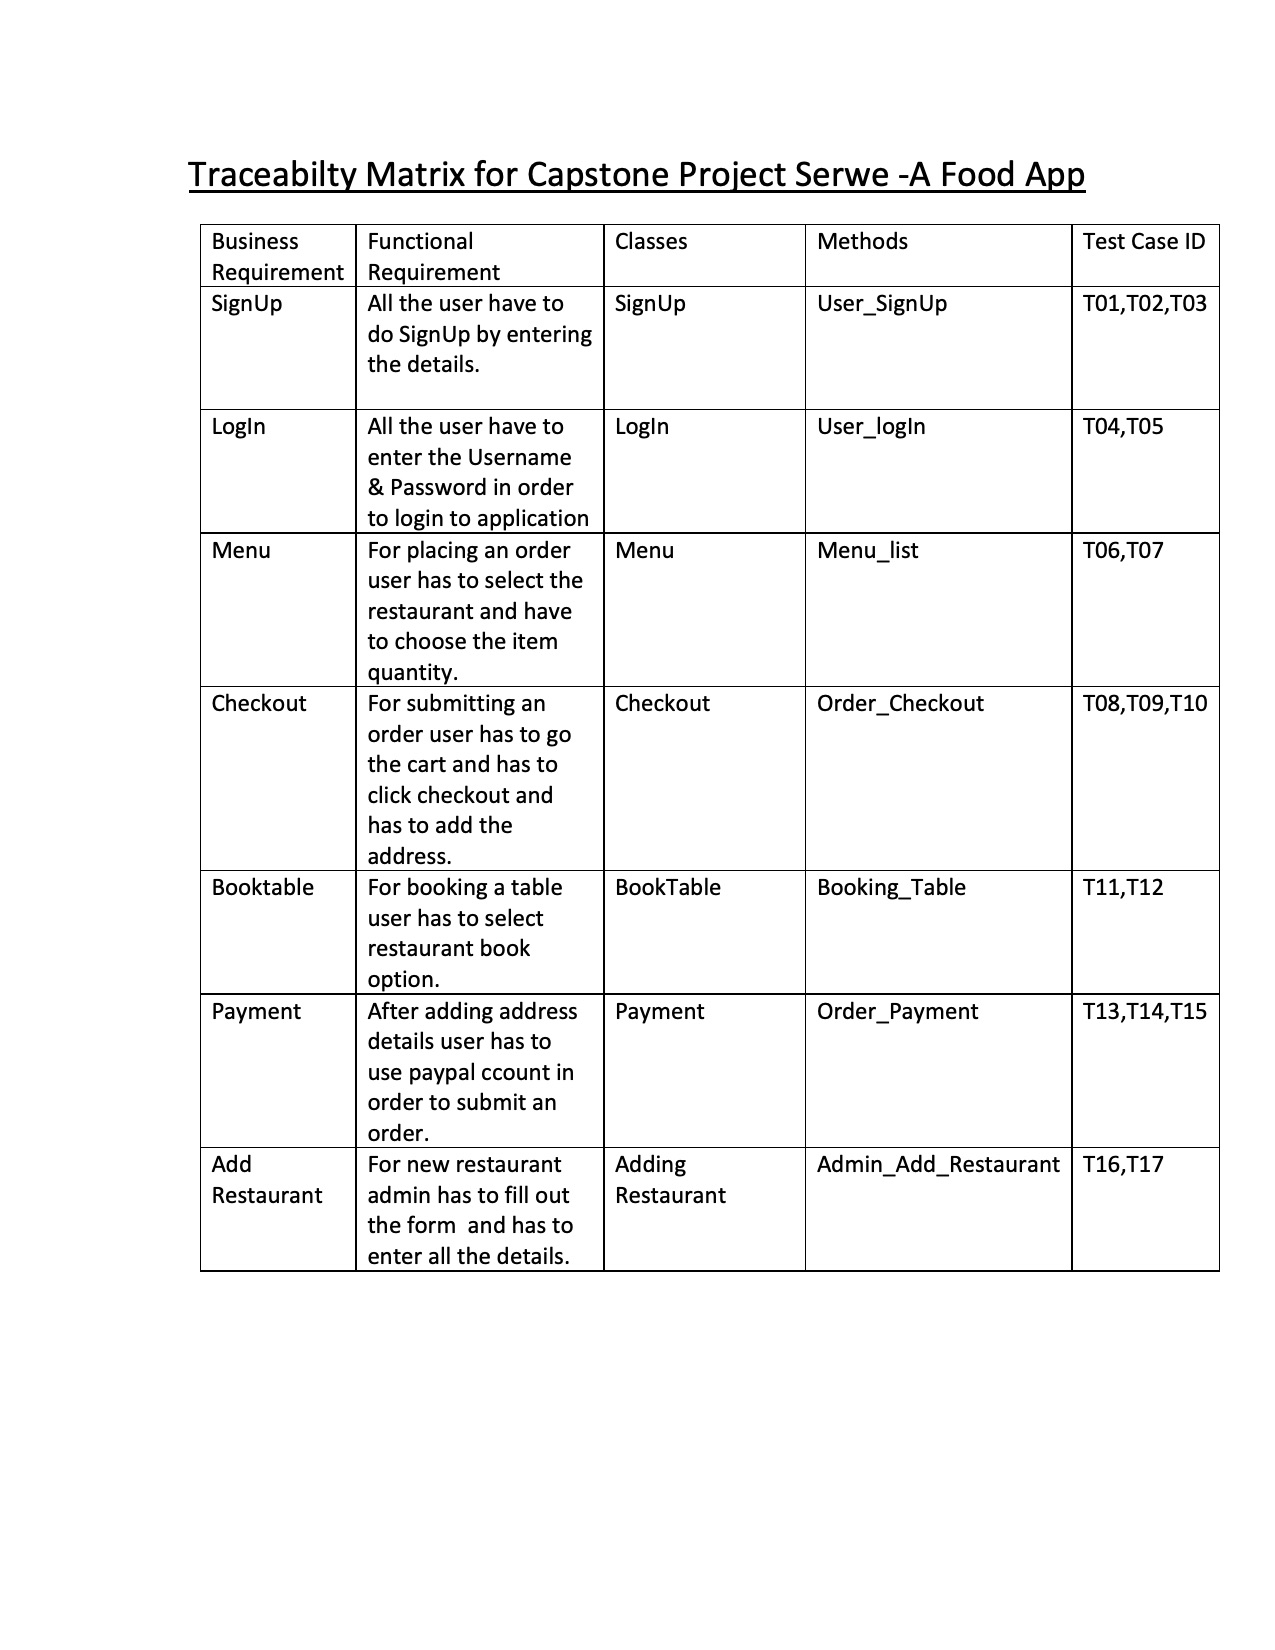
\includegraphics[scale=0.4]{matrix.jpg}
\caption{Admin}

\end{figure}







































\bibliographystyle{abbrv}
\bibliography{main}

\end{document}